%Implementation
\section{Implementation}
\subsection{GUI and IDE}
\subsubsection{Introduction}

The gui and ide are both implemented in JAVA with the JHotDraw 7.1 framework chosen as a basis. The gui was decided early on to function like other popular tools for drawing state charts such as Visio, IBM's Rational software, and Dia. All of these tools choose to be interactive in the drawing phase rather than compile a graph in post. The reason for enforcing interactive drawing is that this tool is design to simplify the original implementation of ladder logic, and building it on a textual graphical language will significantly hurt the primary goal of ease of use. Secondly JAVA was chosen for portability as it was simplier to test one deployment version than multiple ports for the short duration of this project.

The gui itself remains minimal %refer to figure
there is a simple toolbar in which objects can be selected from the pallete and drawn. Properties of an object are directly editable on the object itself %ref figure
instead of the original design of a seperate property palette. Again this design descision was chosen as it is simpler and more immediately understandable by the user.

%figure goes here
\subsubsection{Using The Gui: Parts of the Gui}

\subparagraph{The Main Canvas}

\begin{figure}[htp]
    \centering
    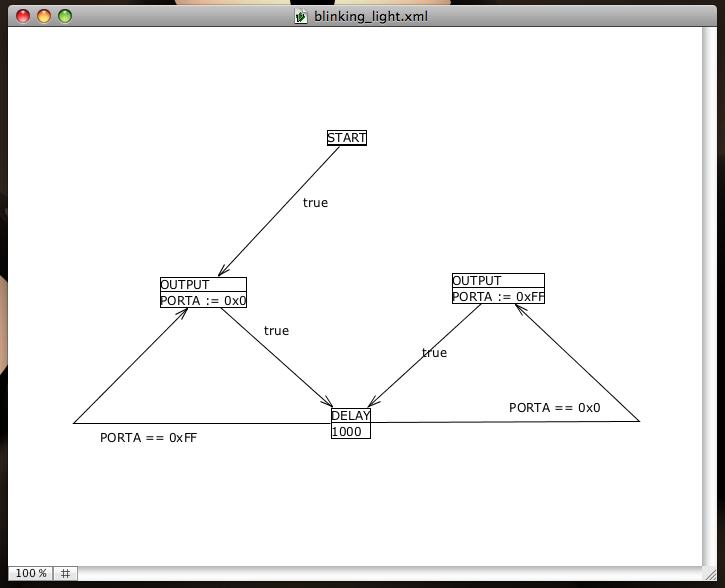
\includegraphics[width=\imgmedium]{./images/plcedit_canvas.png}
    \caption{The Drawing Canvas}
    \label{fig:plcedit_canvas}
\end{figure}

The main canvas represents the main working area for the user as shown in figure \ref{fig:plcedit_canvas}. As one would expect the canvas can be scrolled by using the horizontal and vertical scroll bars. In addition the drawing can also be zoomed in and out by using the zoom keys located at the bottom of the canvas. Object manipulation is accomplished by selecting the appropreate tool from the tools palette then performing the movement with the mouse onto the main drawing canvas.

\subparagraph{The Tools Palette}

\begin{figure}[htp]
    \centering
    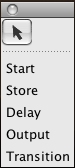
\includegraphics[width=50px]{./images/plcedit_tools.png}
    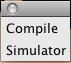
\includegraphics[width=50px]{./images/plcedit_actions.png}
    \caption{The Tools Pallette}
    \label{fig:plcedit_tools}
\end{figure}

The tools pallate is were the user selects their tool to use on the canvas shown in figure \ref{fig:plcedit_tools}. Only one tool can be used at a time. All tools except for compile and simulation are selected on click. Compile and Simulaiton are immediately executed on click.
%TODO: Add simulation tool
The tools listed on the tool pallate are as shown in figure %create figure tool pallate
and have the functionality as follows
\begin{itemize}
\item \textbf{Selection Tool}: This tool allows you to select one or multiple objects. Or edit properties of objects. You can move the object around the canvas by first selecting the object with a single click, then clicking and draging the object to the desired location. Editing properties are accomplished by double clicking the property you would like to edit.
\item \textbf{Transition Tool}: This tool draws transitions between one block to another. Before you draw a transition you must have created the two blocks you wish to connect. To draw the transition you start by clicking and holding down the left mouse button over the starting block then dragging until the line snaps over the ending block. On release of the left mouse button a transition is formed and the two blocks are linked. For layout purposes you may also double click on a transition  line to add more anchors.
\item \textbf{The Start Tool}: A start block is a special tool. The code will give a compile error if more than one start block is placed on the diagram. Start blocks have no other data accociated with them but they serve as the starting point of your program when the PLC unit is first turned on. Your diagram must contain exactly one start block and there must only be one edge leaving the start block. No variables or guard conditions can be evaluated at the start of the program since the controller is still uninitialzied so the result of the guard conditions is entirely dependent on what the chip has at these memory locations.
 %ref figure
\item \textbf{The StoreBlock Tool}: Store blocks are fundemental input blocks. You can use these blocks to perform calculations or update internal variables. To begin drawing a store block you first select this tool. Then you click on the canvas where you would like it to appear. Store blocks are auto-resizing objects thus the size is determined by the content. To edit each field in a store block you double click the parameter you wish to edit. If you wish to delete a line you can simple erase the identifier. If you wish to add a new line change the last identifier to something other than the default placeholder value. A new placeholder will be created as soon as you perform this action in order to allow you to add more lines.
\item \textbf{The Delay Tool}: Delay blocks are used to insert a specified delay into your program the length of the delay is specified in milliseconds. When an edge is taken to the delay block the code execution is delayed and none of the departing edges are taken until the delay time specified has elapsed. It is often useful to have your program wait for a specified period, although the same can be achieved by using a store block and a counter update it is far easier and more precise to use the dedicated delay block.
\item \textbf{The Output Tool}: Output blocks are used to send outputs from the program to pins on the PLC itself. Depending on the chip type there can be one or many different output ports. Each port is a 8-bit representation of the pins, an expression is also allowed on the right hand side so masking would be permitted.
%% TODO: Implement this
\item \textbf{The Input Tool}: Similar to the format of the output block the input block allows you to read data from one or many ports (depending on chip) into an internally used variable.

\item \textbf{Compile Action}: Executing the compile action will start the compilation process into PLC \emphasize{IL} (Intermediate Language) code this code is directly loadable onto the PLC targets to be run. The generated code can then be copied into your PLC's compilation enviroment for run.

\item \textbf{Simulator Tool}: The simulator action brings up a tracing and debugging window. This window allows you to step through each of the code blocks to simulate what might happen as your program runs.
\end{itemize}

\subparagraph{Compile Preview Window}
\begin{figure}[htp]
    \centering
    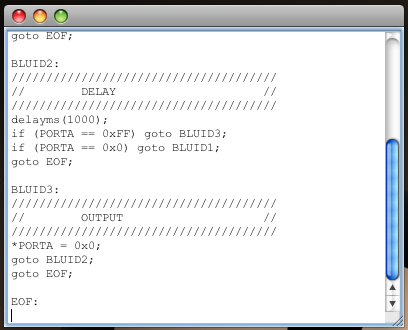
\includegraphics[width=\imgmedium]{./images/plcedit_compile.png}
    \caption{Compile Preview Window}
    \label{fig:plcedit_compile}
\end{figure}

After the compile button is invoked the compile preview window is presented as shown in figure \ref{fig:plcedit_compile}. The preview window serves as a quick overview of the program code that can be loaded onto the device. The user then has the option of saving the text off to a compilable file for loading onto the device.

\subparagraph{Simulator Window}

In order to aid in debugging a simulator mode has been added to the visual editor. When the simulator window is brought up it helps the programmer visually identify what their current memory layout looks like as well as which block they are currently executing. In figure \ref{fig:plcedit_simulator_start} the following view is presented right after the simulator button has been pressed. Note at any point in time the contents of all variables and all ports are shown. Not the start block is automatically highlighted and the ports are initialized to their starting values.

\emphasize{Step Once} allows the user to to step through the current block one step at a time. \emphasize{Step Next} finished all operations in the current block and jumps directly to the next block. Figure \ref{fig:plcedit_simulator_running} demonstrates what the program might look like after a it is allowed to run a few steps.

\begin{figure}[htp]
    \centering
    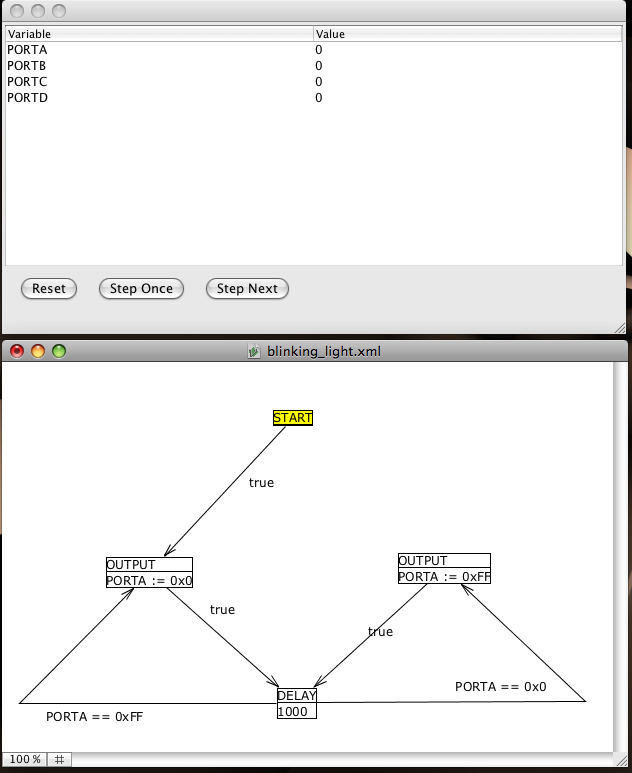
\includegraphics[width=\imgmedium]{./images/plcedit_simulator_start.png}
    \caption{Simulator Window Starting Configuration}
    \label{fig:plcedit_simulator_start}
\end{figure}



\begin{figure}[htp]
    \centering
    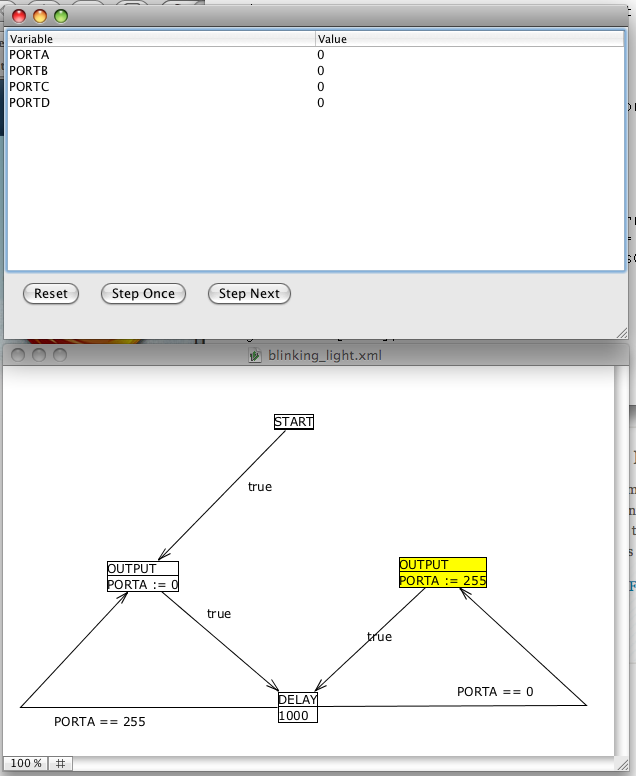
\includegraphics[width=\imgmedium]{./images/plcedit_simulator_running.png}
    \caption{Simulator Window Program Running}
    \label{fig:plcedit_simulator_running}
\end{figure}





\subsection{Data Flow}
%data flow diagram
Construction of the final compiled code starts at the gui level. The GUI composed of tools and drawing elements forms the basis of a directed graph with data. The directed graph forms the basis of our code structure. In each node contains a small ability to have sequential code. The edges allow different sequences of nodes to be executed with logic.

\subsection{Structure}
The structure of each compiled section was carefully constructed to preserve the structure of the drawn graph as closely as possible. The basic structure of each compiled block can be seen as follows:

\begin{definition}
\label{def:genCodeStruct}
Structure of \plcchart \  generated code

\begin{lstlisting}
BLUID5:
//////////////////////////////////
//// Block Header               //
//////////////////////////////////
(Program Code)

if ( guard condition ) goto BLUID2;
goto EOF;
\end{lstlisting}
\end{definition}

As you can observe from definition \ref{def:genCodeStruct} each code block generation first starts with a \emphasize{BLUID} (Block Unique Identifier). The purpose of the \emphasize{BLUID}'s is to give a reference point for the start of the block having a \emphasize{BLUID} label for each block enables any block to connect an edge to it should it choose. The block header which comes right after is an identifier to the type of block being generated. 

In the "(Program Code)" section of the definition \ref{def:genCodeStruct} sits the generated \emphasize{IL} code. This code is the same for each target platform. Each \emphasize{IL} target will have apropreate drivers that will support all the primitives that that \emphasize{IL} will require. These primatives can be found in section \ref{sec:IL}. The code here will resemble C code with specific calls to lower level functions that are supported by the PLC target's drivers.

The final block of if statements impliment the edges leaving the block. Each edge is guarded by an if statement, and will have the goto portion point the the correct \emphasize{BLUID} as specified by the diagram.

If at any point no edges are valid the the program will terminate by going to the label "EOF" which will be located at the end of the file.
%alternative return statement.

\subsection{Compilation}
Each of the blocks will compile their own snippets of code the translation is as follows:

\begin{definition}
\label{def:startblock}
(The start block generate no program code it's only represented as a block so we may traverse along it's edges)
\end{definition}

